%\documentclass{article}
%\usepackage{pgfgantt}

\begin{document}

In the following chapter the initial and final Gantt charts will be shown as well as the risk plan that was developed during the project. 
\subsection{Gantt chart}
\begin{center}
  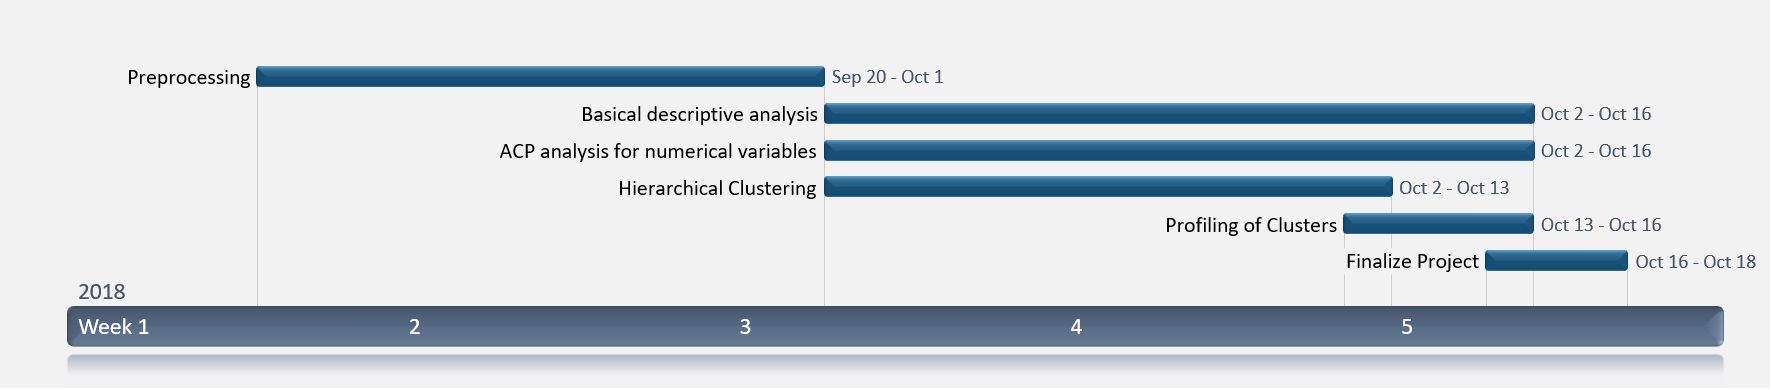
\includegraphics[height=5cm, width=13cm]{images/initial_guntt_chart.png}
  \captionof{figure}{Initial Gantt chart}
  \label{fig:gunttinitial}
\end{center}
As shown in figure ~\ref{fig:gunttinitial} we tried to finish the work seven days before the actual deadline on the 26th of October. This time was planned to buffer eventualities like persons leaving the course or other not planned things that will increase the time needed to finish. In the beginning the whole team works on the pre-processing, since it is needed for all following steps. After the pre-processing the tasks have been split between the different members of the group. Teams out of two people have been formed and assigned to one of the following tasks:
\begin{enumerate}
\item Basic descriptive analysis
\item PCA for numerical variables
\item Hierarchical clustering
\end{enumerate}
The first task for the basic descriptive analysis was assigned to Roland Frieß and Enrique Gonzalez. The PCA of numerical variables was assigned to Jordi Armengol and Marc Catrisse. The hierarchical clustering was scheduled for Albert Figuera and Jacobo Moral. Since the hierarchical clustering is needed to profile the clusters, Albert and Jacobo are also doing the profiling of the clusters. After that the project will be finalized. The finalization includes a feedback-circle in which the groups give feedback to each other. So after getting the feedback from the other group each group implemented the feedback given to them. The finalization also contains including the plots in the final essay and writing it. 


\begin{center}
  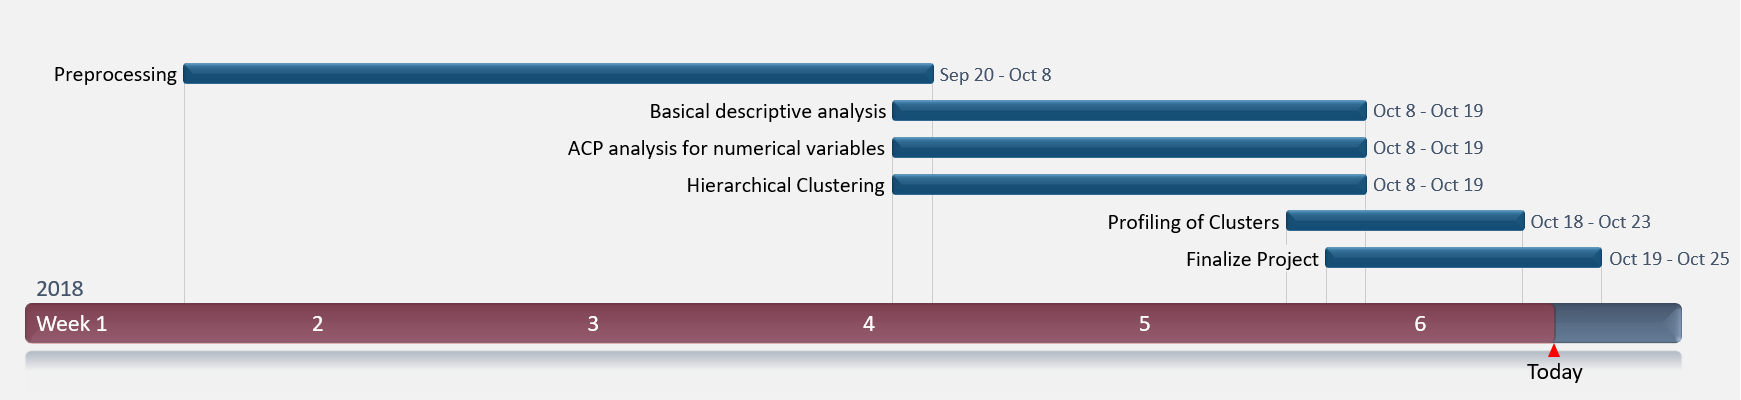
\includegraphics[height=4.5cm, width=13cm]{images/final_gunnt_chart.png}
  \captionof{figure}{Final Gannt chart}
  \label{fig:gunttfinal}
\end{center}
In the final Gannt chart we changed the time for the profiling of the clustering, and added more time to develop our project. We did not think we would need that much time to finalize the project. But since the writing and documentation takes more time than expected, we added more time for the finalization of the project. 


%\begin{center}
%      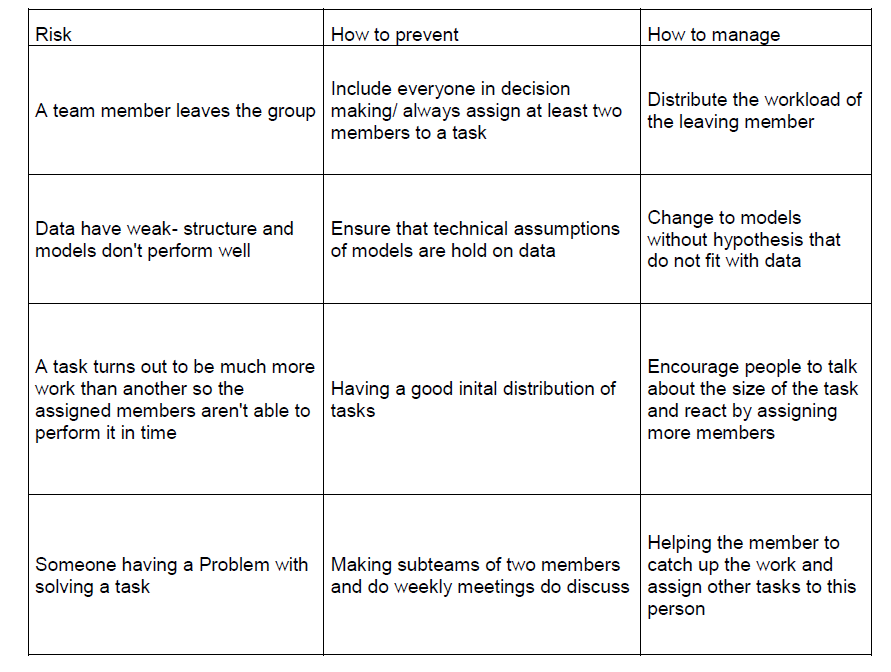
\includegraphics[height=10cm, width=10cm]{images/Riskplan.PNG}
%  \captiononof{Risk plan}
%  \label{fig:riskplan}
%\end{center}


\begin{comment}
\begin{table}[!h]
\caption{Risk Plan}
\label{T:riskplan}
\begin{tabular}{| l | l | l |}
\hline
\cline{1-6}
\textbf{Risk} & \textbf{How to prevent} & \textbf{How to manage} \\
\hline

 A team member leaves the group & include everyone in decision making \\and always assign at least two members\\ to a task &Distribute the workload \\of the leaving member \\ \hline
 
 
  Data have weak- structure \\and models don't perform well & Ensure that technical assumptions\\ of models are hold on data  & Change to models without hypothesis that do not fit with data \hline
  
  
  A task turns out to be much more\\ work than another \\so the assigned members aren't \\able to perform it in time& Having a good inital distribution of tasks &Encourage people to talk about the size of the task and react by assigning more members  \\ \hline
  
  
  Someone having a Problem \\with solving a task& Making subteams of two members\\ and do weekly meetings do discuss &  Helping the member to catch up \\the work and assign other tasks\\ to this person\\ \hline



\end{tabular}
\end{table}

\end{comment}

\subsection{Final tasks assignment grid}

\begin{table}[H]
\begin{tabular}{|l|l|l|l|l|l|l|}
\hline
Participant                                       & Jordi & Marc & Albert & Roland & Enrique & Jacobo \\ \hline
Motivation of the work and general description    &   X   &          &      &      &         &        \\ \hline
Data Source presentation                          &      &     X     &   X    &      &       &    X    \\ \hline
Formal description of Data structure and metadata &      &          &   X    &      &        &    X    \\ \hline
Data Mining process performed                     &      &     X     &       &     &     X     &        \\ \hline
Preprocessing                                     &   X   &     X     &      &   X   &          &        \\ \hline
Basic statistical descriptive analysis            &      &          &       &  X    & X        &        \\ \hline
ACP analysis for numerical variables              & X    &  X        &       &      &          &        \\ \hline
Clustering                                        &      &          &   X    &     &          &    X    \\ \hline
Profiling                                         &      &          &   X    &      &          & X      \\ \hline
Conclusions                                       & X    &         &      &     &          &      \\ \hline
Working plan                                      &      &          &     &   X   &          &        \\ \hline
Final Report                                      &  X   &  X       &   X   &   X   &  X       &   X     \\ \hline
\end{tabular}
\end{table}

\subsection{Risks and deviances in scheduling}

In order to be prepared for different situations that can endanger the success of the project we developed a risk plan. In the risk plan we identified different risks and found ways to prevent the risk and manage the different scenarios.% ~\ref{fig:riskTable}.

\begin{table}[H]
\centering
\begin{tabular}{|p{.3\textwidth}|p{.3\textwidth}|p{.3\textwidth}|}
\hline
Risk                                                   & How to prevent                                  & How to manage                                         \\ \hline

A team member leaves the group & Include everyone in decision making and always assign at least two members to a task & Distribute the workload of the leaving member \\ \hline

Data have weak- structure and models don't perform well & Ensure that technical assumptions of models are hold on data  & Change to models without hypothesis that do not fit with data \\ \hline

A task turns out to be much more work than another so the assigned members aren't able to perform it in time & Having a good initial distribution of tasks & Encourage people to talk about the size of the task and react by assigning more members \\ \hline
  
  
 Someone having a problem with solving a task& Making sub-teams of two members and do weekly meetings do discuss &  Helping the member to catch up the work and assign other tasks to this person \\ \hline

\end{tabular}
\caption{Project risk table}
\label{fig:riskTable}
\end{table}

Our main self-critical point about the deviances of the final scheduling with respect to the originally designed one, the main problem is that we underestimated the amount of work that would suppose the pre-processing. It took longer than expected, and this problem affected the rest of the project, because many tasks depended on this one. Also, the pre-processing is not quite parallelizable. Two different sub-teams could be doing PCA and clustering, respectively, but it was not feasible to divide the pre-processing into different sub-teams.

Although this risk had been considered in the risk plan, it could not be prevented, because it hit as at the beginning, Fortunately it could me managed properly, by meeting two members of the team and doing it (so, adding more people to the task).
\end{document}